\chapter{Introduction}
Object-Centric Process Mining (OCPM) was introduced to analyze processes that involve multiple interacting objects.
Traditional process mining techniques cannot capture these interactions because they require event logs to be flattened into a case-centric structure, which removes the relations between objects.
OCPM avoids this limitation and makes it possible to represent and analyze complex real-world behavior that depends on the interaction of several objects at the same time.

Although interest in OCPM continues to grow, applying the latest OCPM tools proposed in research remains difficult in practice.
The current tool landscape is fragmented since most tools implement only a single functionality and require their own setup and maintenance.
This limits the ability of practitioners to apply OCPM in real settings.
Solutions from traditional process mining that were designed to address similar issues, such as ProM~\cite{prom}, have not been widely adopted in the object-centric context.
As a result, developers often need to build their tools from the ground up.
This makes it challenging for researchers and practitioners to reuse existing work or to develop more advanced analyses.
It also makes it hard to provide tool support for users with little software development experience.
These challenges motivate the search for a unified and extensible approach to research tool development in OCPM.

To address these challenges, this thesis proposes a unified and extensible approach by introducing Ocelescope, a web-based framework that offers core functionality and supports extensibility through two methods:
\begin{itemize}
	\item a \textbf{plugin system} that enables simple OCPM applications to be loaded at runtime within a single running instance of Ocelescope;
	\item a \textbf{module system} that allows developers to use Ocelescope as the foundation for custom OCPM tools without reimplementing standard functionality, while benefiting from an easy setup process.
\end{itemize}
Together, these mechanisms allow smaller tools to be implemented as plugins in a more specialized and modern environment than ProM~\cite{prom}. More complex tools can build on the module system so that developers can focus on their specific analysis tasks instead of creating the entire tool infrastructure from scratch.

To assess the effectiveness of the framework, two user studies were conducted. The first study examined how end users interact with Ocelescope and its standard functionality. The second study focused on the experience of developers who implemented plugins. In addition, two proof-of-concept plugins were created to demonstrate the feasibility of integrating existing OCPM methods. The results indicate that users can work with the framework efficiently and that developers can extend it with relatively little effort. This suggests that Ocelescope can improve tool support in OCPM.

The remainder of this chapter is structured as follows. In \cref{sec:intro_ssec:motiv}, we motivate the need for unified and extensible tool support. In \cref{sec:intro_ssec:probs}, we define the problem addressed in this thesis. The research questions are presented in \cref{sec:intro_ssec:RQs}, and the goals of the thesis are described in \cref{sec:intro_ssec:goals}.

\section{Motivation}
\label{sec:intro_ssec:motiv}

Since the introduction of OCPM, a growing number of research tools have been developed to support its use.
These tools span a wide range of formats, including standalone Python scripts (e.g., \textit{TOTem}~\cite{totem}, \textit{Super Variants}~\cite{supervariants}), web-based applications (e.g., \textit{OC$\pi$}~\cite{ocpi}, \textit{OCPQ}~\cite{ocpq}, \textit{ProAct}~\cite{proact}), and ProM plugins (e.g., \textit{Object-Centric Local Process Models}~\cite{oclpm}). While this tool landscape reflects increasing interest in OCPM, it also highlights several practical limitations that hinder broader adoption.

Many existing tools are implemented as ad-hoc prototypes that lack documentation, reproducibility, or long-term maintenance. They are often abandoned after their initial publication. Script-based tools in particular require expert knowledge to install and execute. They are rarely packaged in a structured manner and often suffer from dependency and reproducibility issues, as limited effort is invested in making their execution environments reliable and repeatable. Tools with graphical user interfaces frequently reimplement basic functionality such as importing and exporting logs, providing log overviews, filtering data, and generating visualizations. Examples of this can be observed across multiple tools, as shown in Figure~\ref{fig:three}.

\begin{figure}[htbp]
	\centering
	\begin{subfigure}[b]{0.3\textwidth}
		\centering
		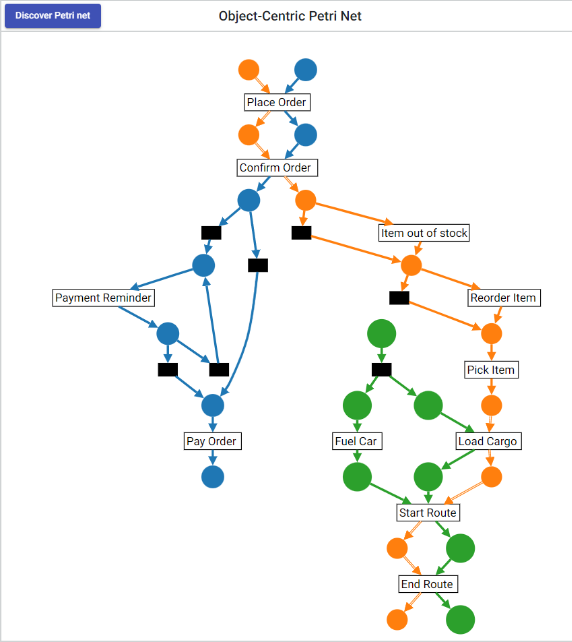
\includegraphics[width=\textwidth]{figures/motivation/petri_ocpi.png}
		\caption{OC$\pi$~\cite{ocpi}}
		\label{fig:sub1}
	\end{subfigure}
	\hfill
	\begin{subfigure}[b]{0.3\textwidth}
		\centering
		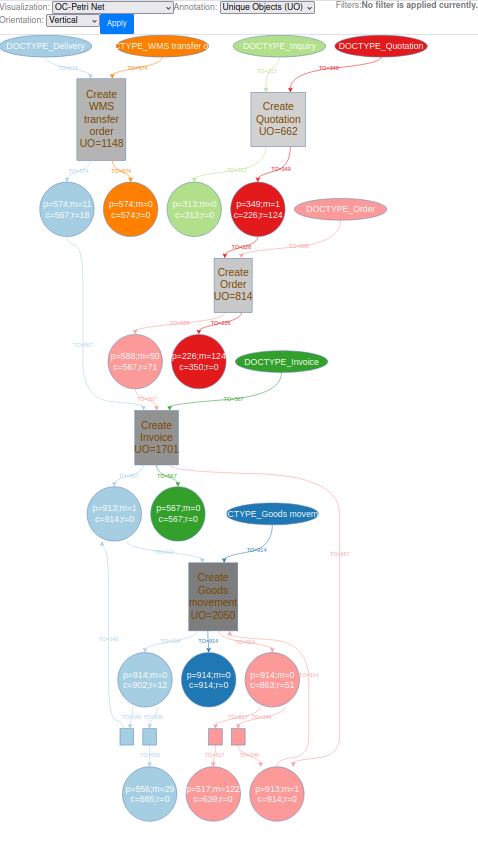
\includegraphics[height=1.1\textwidth]{figures/motivation/petri_ocpm.png}
		\caption{OC-PM~\cite{ocpm}}
		\label{fig:sub2}
	\end{subfigure}
	\hfill
	\begin{subfigure}[b]{0.3\textwidth}
		\centering
		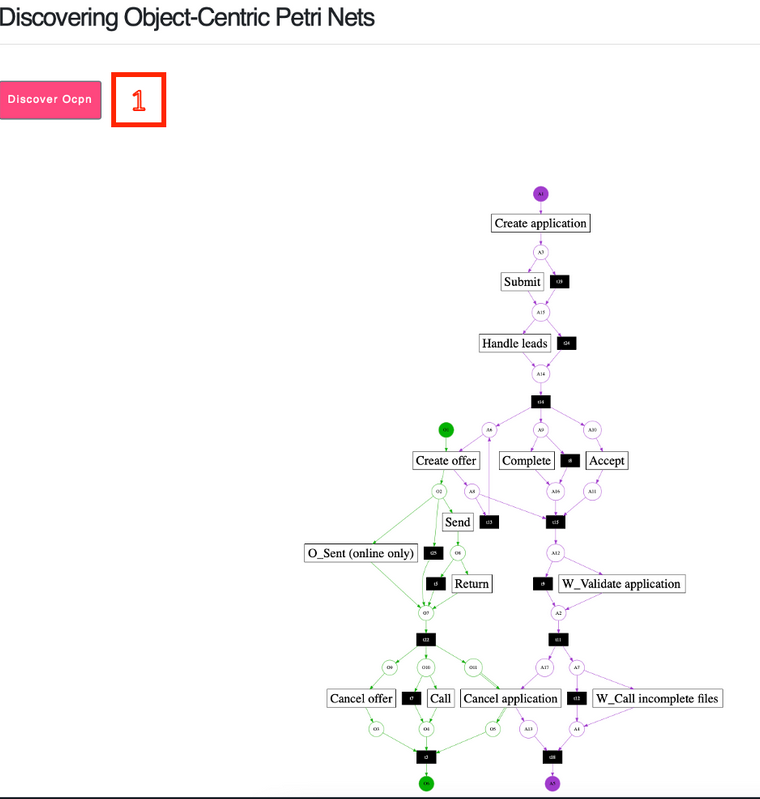
\includegraphics[width=\textwidth]{figures/motivation/petri_opera.png}
		\caption{Opera~\cite{opera}}
		\label{fig:sub3}
	\end{subfigure}
	\caption{Example of redundant implementations of object-centric Petri net visualization across different tools.}
	\label{fig:three}
\end{figure}

Because of this fragmentation, developers spend time on features that are common across tools instead of focusing on their specific contributions.
These problems are common in research software and are not limited to OCPM. ProM, which addressed these challenges in traditional process mining, does not transfer well to OCPM.
It relies on outdated technologies and requires detailed knowledge of its internal architecture to develop or maintain plugins. Developer documentation is limited, which further complicates plugin development. As a result, researchers and practitioners often need to create new solutions from scratch whenever they want to implement their own OCPM functions.

\section{Problem Statement}
\label{sec:intro_ssec:probs}
The current landscape of OCPM tools lacks extensibility, maintainability, and standardization.
Researchers and practitioners who aim to develop or extend such tools are often required to reimplement basic functionality, which leads to redundant effort and makes further development more difficult.
As a result, the field consists of a fragmented collection of single-purpose tools with inconsistent user experiences, varying levels of support, and limited reusability.
This fragmentation creates a significant barrier for both research and practical adoption of OCPM.

\section{Research Questions}
\label{sec:intro_ssec:RQs}

This thesis is guided by the following research questions, which will be addressed in the subsequent chapters:

\begin{description}
	\item[RQ1:] What is the current state of tool support for OCPM?
	      \begin{enumerate}[label=\alph*)]
		      \item Which tools are currently available, and what functionality do they provide?
		      \item Which functionality is commonly reimplemented across these tools?
		      \item Which frameworks, technologies, and libraries form the basis of these tools?
	      \end{enumerate}

	\item[RQ2:] How can an extensible tool architecture for OCPM be designed?
	      \begin{enumerate}[label=\alph*)]
		      \item Which software design principles and patterns support extensibility, maintainability, and reusability?
		      \item How can common functionality be integrated to reduce fragmentation?
	      \end{enumerate}

	\item[RQ3:] How can a tool that realizes the proposed extensible architecture be implemented?
\end{description}

\section{Research Goals}
\label{sec:intro_ssec:goals}

To answer the research questions posed in the previous section, this thesis pursues the following research goals:

\begin{description}
	\item[RG1:] Analyze the current state of tool support for OCPM.
	      \begin{itemize}
		      \item Conduct a systematic literature review on existing OCEL-based tools.
		      \item Analyze the functionality implemented in these tools.
		      \item Identify functionality that is shared or repeatedly implemented across tools.
	      \end{itemize}

	\item[RG2:] Design an extensible tool architecture for OCPM.
	      \begin{itemize}
		      \item Define requirements for extensibility, maintainability, and reusability.
		      \item Develop a concept for a tool architecture that integrates common functionality.
		      \item Identify software design patterns that support modularity and extension.
	      \end{itemize}

	\item[RG3:] Implement a tool that realizes the proposed extensible architecture.
\end{description}

\section{Contributions}

This thesis makes the following contributions to tool support for OCPM by achieving the goals RG1 to RG3.

\begin{itemize}
	\item \textbf{Systematic Literature Review:} A review of 31 publications that introduce OCPM tools, identifying recurring functionality and common limitations.
	\item \textbf{Implementation of Ocelescope:} A web-based framework that provides core functionality for OCPM, including importing and exporting OCEL, inspecting logs, and filtering data.
	\item \textbf{Extension Framework:} A framework for developing extensions for Ocelescope, supported by documentation that describes how to build and use plugins and modules.
	\item \textbf{Evaluation:} An evaluation of Ocelescope and the extension mechanisms through two user studies.
\end{itemize}

\section{Thesis Structure}
\label{sec:intro_ssec:structure}

The remainder of this thesis is structured as follows. An overview of the chapter structure and workflow is illustrated in \Cref{fig:chapter-overview}. \Cref{chap:related_work} reviews extensible software frameworks and tools that can serve as a basis for building OCPM applications and analyzes their strengths and weaknesses. \Cref{chap:prelim} introduces software design patterns and development technologies that support the design of Ocelescope. \Cref{chap:requirements} analyzes the current OCPM tool landscape and derives requirements for extensible tool support. \Cref{chap:design} presents the architecture and overall design of the Ocelescope framework. \Cref{chap:impl} describes the implementation of the framework and its main components. \Cref{chap:eval} evaluates Ocelescope and the development of extensions through two user studies. \Cref{chap:discussion} discusses the results, limitations, and implications of the work. Finally, \Cref{chap:conclusion} summarizes the findings and outlines directions for future research.

\begin{figure}[t]
	\centering
	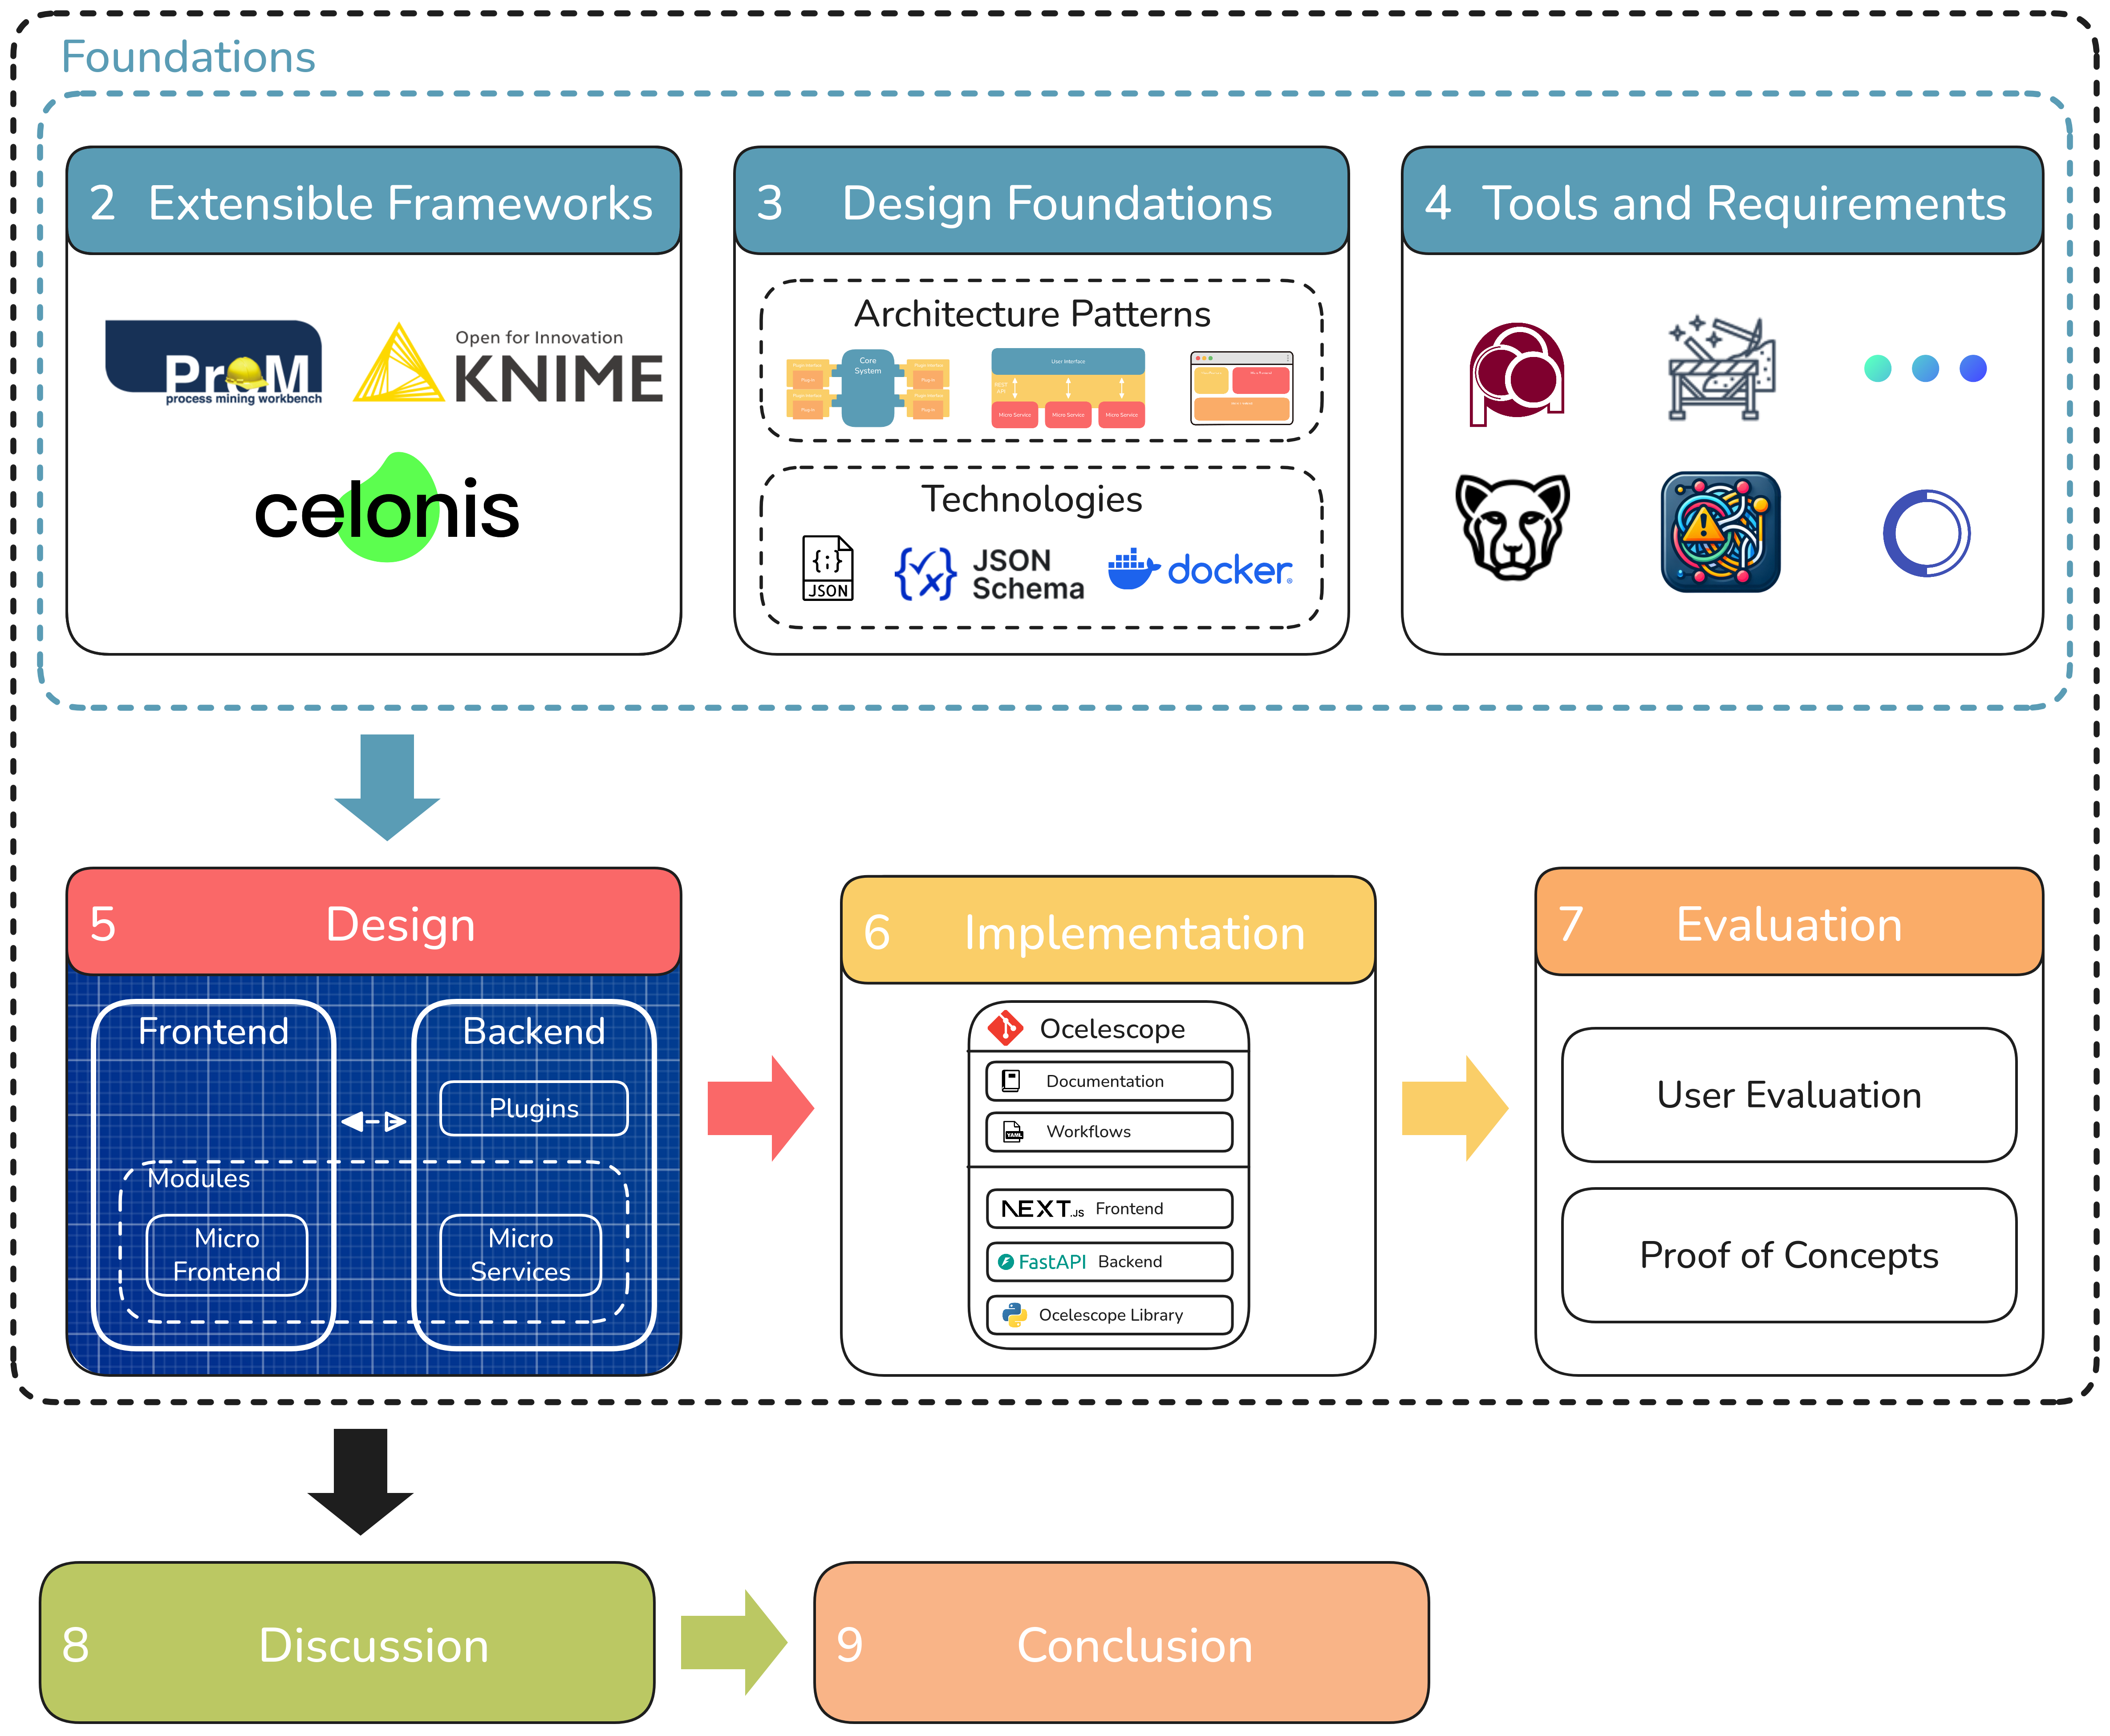
\includegraphics[width=\linewidth]{./figures/introduction/ChapterOverview.png}
	\caption{Chapter overview and development workflow. The work begins with Foundations (Chapters 2--4: Extensible Frameworks, Design Foundations, and Tools \& Requirements), which informs the Design phase (Chapter 5). The design is realized in Implementation (Chapter 6) and assessed in Evaluation (Chapter 7), culminating in Discussion (Chapter 8) and Conclusion (Chapter 9).}
	\label{fig:chapter-overview}
\end{figure}

